
\begin{exercise}{\emph{(2.6 nel testo)}}
  Considerate il modello in cui $Y_1,\ldots, Y_n$ sono indipendenti e
  identicamente distribuite come una uniforme $Y \sim U(0, \theta)$,
  dove $\theta$ \`e il valore massimo che pu\`o assumere $Y$.
  Determinate per simulazione la distribuzione campionaria di $T = 2Y$
  considerando $\theta = 100, n = 20$. Mostrate con un istogramma che
  la distribuzione dello stimatore \`e approssimabile da una
  normale. Qual \`e la varianza di $T$? Usate questa varianza per
  sovrapporre all'istogramma la curva normale che lo approssima
  (ricordate di disegnare l'istogramma in R con l'opzione freq =
  FALSE).
\end{exercise}
Questo il codice che implementa l'esercizio:
\lstinputlisting{r-sources/exercises/chapter-two/two-six.R}
Vediamo qualche risultato inserendo in R:
\begin{lstlisting}
  > twosix()
  $estimatorVector
    [1]  95.96794 105.40497 110.64482  89.14495 107.99978 116.03221
    94.73158 ...
  
  $empiricalMean
  [1] 100.0089

  $empiricalVar
  [1] 166.6052

  $empiricalVarComputedByHand
  [1] 166.6052  
\end{lstlisting}
L'esecuzione della funzione produce la \autoref{fig:two-six}, dove la
curva in blu rappresenta la densit\`a inferita usando gli algoritmi
disponibili in R dello stimatore $2\bar{Y}$, mentre la curva in rosso
rappresenta il modello esatto usando come parametri i valori stimati
dalla media e dalla varianza campionaria (riportate nel precedente
output come \texttt{empiricalMean} e \texttt{empiricalVar}).
\begin{figure}[htb]
\centering
\includegraphics[height=13cm,width=13cm]{r-sources/exercises/chapter-two/two-six.ps}
\caption{Istogramma esercizio 2.6 del testo}
\label{fig:two-six}
\end{figure}
  

